\documentclass[aspectratio=169]{beamer}
\usetheme{Madrid}
\usepackage{graphicx}
\usepackage{booktabs}

\title{Branch Specialization in Attention}
\subtitle{Phase 1 Repeat-Match Causal Ablation Checkpoint}
\author{Research checkpoint}
\date{May 21, 2026}

\begin{document}

\begin{frame}
  \titlepage
\end{frame}

\begin{frame}{Current Question}
  \textbf{Question:} Do structurally corresponding attention heads have stable
  causal functions across random seeds?

  \vspace{0.7em}
  The current concrete target is the early-layer repeat-match role found in
  Pythia-160M. Previous results showed that this role is concentrated and much
  more stable after raw-score head alignment than by same index.

  \vspace{0.7em}
  This checkpoint asks whether those aligned heads are causally important for a
  repeated-token prediction task.
\end{frame}

\begin{frame}{Ablation Design}
  Evaluation sequences:
  \[
    [x_1,\ldots,x_{32},x_1,\ldots,x_{32}]
  \]

  \vspace{0.5em}
  Loss is scored on second-half continuation positions \(x_i \rightarrow x_{i+1}\).
  The same 64 synthetic sequences are reused across all nine seeds.

  \vspace{0.5em}
  Ablation zeros selected per-head attention outputs before the GPT-NeoX
  attention output projection.
\end{frame}

\begin{frame}{Conditions}
  \begin{itemize}
    \item \textbf{own top}: target seed's top repeat-match heads in layers 0--1.
    \item \textbf{own random}: random same-layer controls, excluding top heads.
    \item \textbf{same index}: another seed's top head indices ablated in the target.
    \item \textbf{aligned}: another seed's top heads mapped into the target by
      raw-score Hungarian alignment.
  \end{itemize}

  \vspace{0.6em}
  Positive loss delta means the ablation made repeated-token prediction worse.
\end{frame}

\begin{frame}{Aggregate Result}
  \centering
  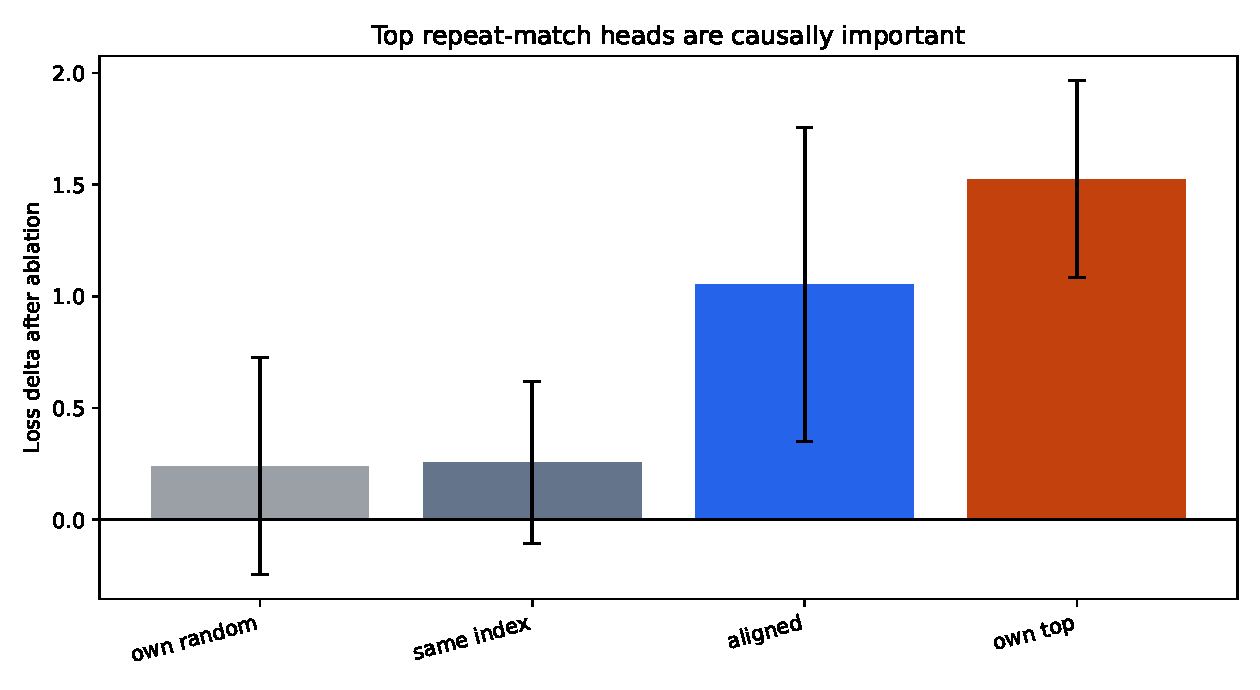
\includegraphics[width=0.88\linewidth]{figures/condition_loss_delta.pdf}
\end{frame}

\begin{frame}{Numerical Summary}
  \begin{table}
    \centering
    \begin{tabular}{lrr}
      \toprule
      Condition & Mean loss delta & Mean target-logit delta \\
      \midrule
      own random & 0.2403 & -0.7184 \\
      same index & 0.2571 & -0.7014 \\
      aligned & 1.0538 & -1.5750 \\
      own top & 1.5244 & -2.0689 \\
      \bottomrule
    \end{tabular}
  \end{table}

  Aligned transferred heads are far closer to own-top heads than to same-index
  or random controls.
\end{frame}

\begin{frame}{Transfer Test}
  \centering
  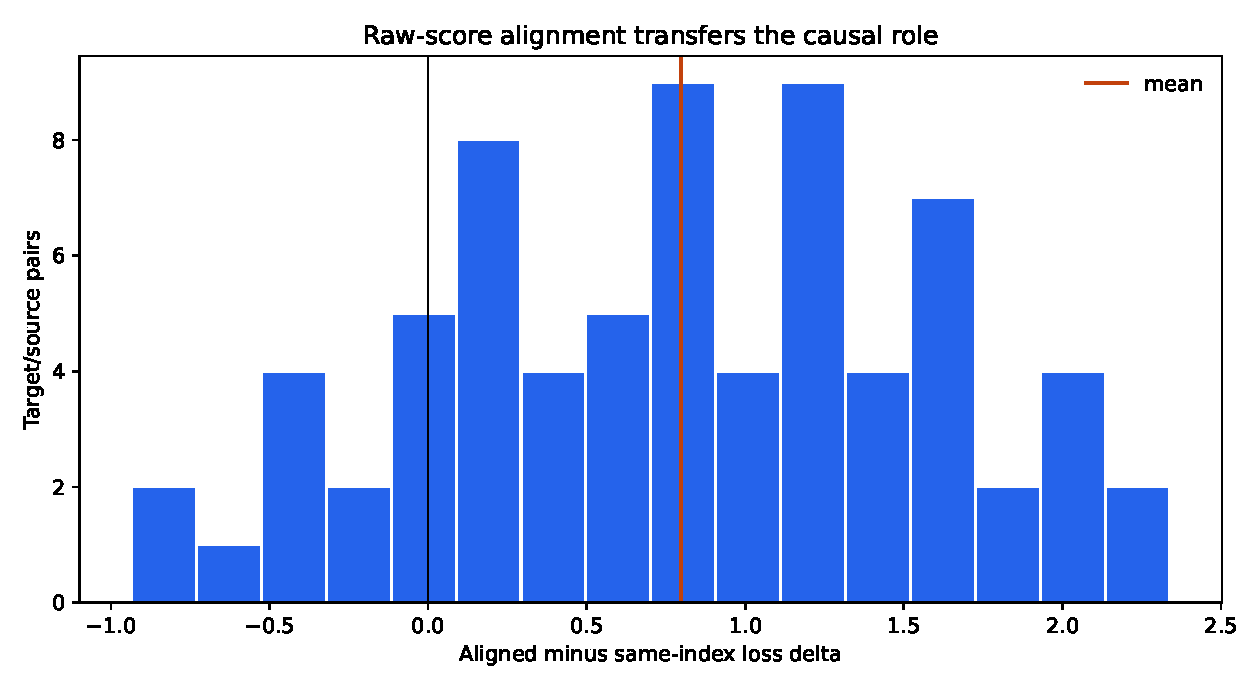
\includegraphics[width=0.88\linewidth]{figures/paired_transfer_difference.pdf}

  \vspace{0.4em}
  Paired aligned-minus-same-index mean loss difference: \(0.7967\);
  positive in \(59/72\) target/source pairs.
\end{frame}

\begin{frame}{Own-Seed Causal Check}
  \centering
  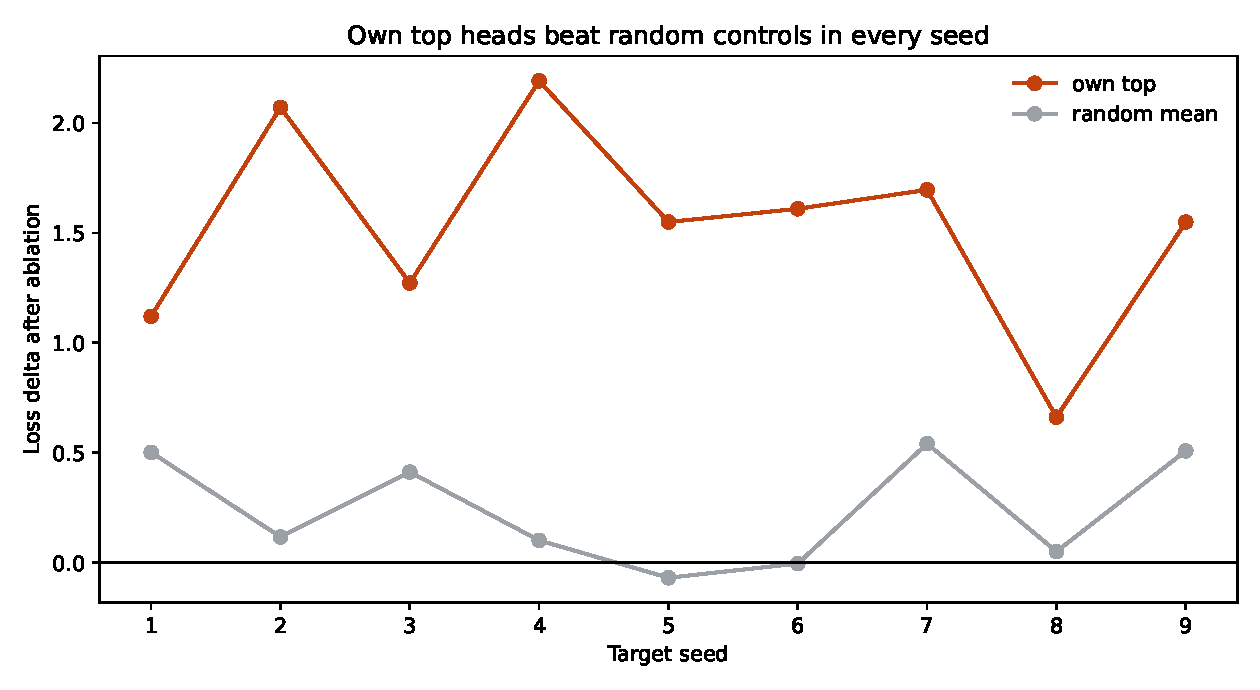
\includegraphics[width=0.88\linewidth]{figures/own_top_vs_random_by_seed.pdf}

  \vspace{0.4em}
  Own top heads beat each seed's random-control mean in \(9/9\) seeds.
\end{frame}

\begin{frame}{Interpretation}
  Findings:
  \begin{itemize}
    \item Repeat-match heads are causally relevant on this synthetic task.
    \item Same layer/head index is a poor cross-seed transfer rule.
    \item Raw-score alignment transfers the causal role much better.
  \end{itemize}

  \vspace{0.6em}
  Stronger claim not yet established:
  \begin{itemize}
    \item This does not yet test heterogeneous branch architectures.
  \end{itemize}
\end{frame}

\begin{frame}{Decision}
  Continue with repeat-match / induction-style behavior as the first causal
  test bed.

  \vspace{0.8em}
  Next step:
  \begin{itemize}
    \item build or adapt a small branched-attention training setup;
    \item vary branch structure or structural heterogeneity;
    \item measure raw-score alignment, role specialization, and causal ablation
      with the same pipeline.
  \end{itemize}
\end{frame}

\begin{frame}{Provenance}
  \begin{itemize}
    \item Script: \texttt{scripts/repeat\_match\_ablation.py}
    \item Output: \texttt{results/phase1\_repeat\_match\_ablation\_pythia160m}
    \item Report: \texttt{doc/phase1\_repeat\_match\_ablation\_pythia160m.md}
    \item Role input: \texttt{results/phase1\_pythia160m\_attention\_role\_specialization}
    \item Alignment input: \texttt{results/phase0\_pythia160m\_seed1\_to\_9\_step143000\_raw\_scores}
    \item Data copied into this deck folder under \texttt{data/}
  \end{itemize}
\end{frame}

\end{document}
